\documentclass{article}

% Packages for formatting
\usepackage[margin=1in]{geometry}
\usepackage{fancyhdr}
\usepackage{enumerate}
\usepackage{graphicx}
\usepackage{kotex}
\usepackage{amsmath}
\usepackage{amsthm}
\usepackage{algorithm2e,setspace}
\usepackage{algpseudocode}
\usepackage{xcolor}
\usepackage{amssymb}

% Fonts
\usepackage[T1]{fontenc}
\usepackage[utf8]{inputenc}
\usepackage{newpxtext,newpxmath}
\usepackage{sectsty}

% Define colors
\definecolor{blue1}{HTML}{0077c2}
\definecolor{blue2}{HTML}{00a5e6}
\definecolor{blue3}{HTML}{b3e0ff}
\definecolor{blue4}{HTML}{00293c}
\definecolor{blue5}{HTML}{e6f7ff}

\definecolor{thmcolor}{RGB}{231, 76, 60}
\definecolor{defcolor}{RGB}{52, 152, 219}
\definecolor{lemcolor}{RGB}{155, 89, 182}
\definecolor{corcolor}{RGB}{46, 204, 113}
\definecolor{procolor}{RGB}{241, 196, 15}

\usepackage{color,soul}
\usepackage{soul}
\newcommand{\mathcolorbox}[2]{\colorbox{#1}{$\displaystyle #2$}}
\usepackage{cancel}
\newcommand\crossout[3][black]{\renewcommand\CancelColor{\color{#1}}\cancelto{#2}{#3}}
\newcommand\ncrossout[2][black]{\renewcommand\CancelColor{\color{#1}}\cancel{#2}}

\usepackage{hyperref}
\usepackage{booktabs}

% Chapter formatting
\definecolor{titleblue}{RGB}{0,53,128}
\usepackage{titlesec}
\titleformat{\section}
{\normalfont\sffamily\Large\bfseries\color{titleblue!100!gray}}{\thesection}{1em}{}
\titleformat{\subsection}
{\normalfont\sffamily\large\bfseries\color{titleblue!50!gray}}{\thesubsection}{1em}{}

%Tcolorbox
\usepackage[most]{tcolorbox}

%Tikzpicture
\usepackage{tikz-cd}
\usetikzlibrary{positioning}
\usetikzlibrary{angles, quotes}

% Header and footer formatting
\pagestyle{fancy}
\fancyhead{}
\fancyhf{}
\rhead{Student ID: 20192250\quad Name: 지용현}%\rule{3cm}{0.4pt}}
\lhead{\textcolor{blue2}{\textbf{CA Assignment \#3}}}
% Define footer
\newcommand{\footer}[1]{
	\begin{flushright}
		\vspace{2em}
		\includegraphics[width=2cm]{school_logo.jpg} \\
		\vspace{1em}
		\textcolor{blue2}{\small\textbf{#1}}
	\end{flushright}
}
%\rfoot{\large Department of Information Security, Cryptogrphy and Mathematics, Kookmin Uni.\includegraphics[height=1.5cm]{school_logo.jpg}}
\fancyfoot{}
\fancyfoot[C]{-\thepage-}

\newcommand{\ie}{\textnormal{i.e.}}
\newcommand{\rsa}{\mathsf{RSA}}
\newcommand{\rsacrt}{\mathsf{RSA}\textendash\mathsf{CRT}}
\newcommand{\inv}[1]{#1^{-1}}

\usepackage{amsthm}
\newtheorem{axiom}{Axiom}[section]
\newtheorem{theorem}{Theorem}
\newtheorem*{theorem*}{Theorem}
\newtheorem{proposition}[theorem]{Proposition}
\newtheorem{corollary}{Corollary}[theorem]
\newtheorem*{corollary*}{Corollary}
\newtheorem{lemma}[theorem]{Lemma}
\newtheorem*{lemma*}{Lemma}

\theoremstyle{definition}
\newtheorem{definition}{Definition}
\newtheorem*{definition*}{Definition}
\newtheorem{remark}{Remark}
\newtheorem{exercise}{Exercise}[section]

%New Command
\newcommand{\set}[1]{\left\{#1\right\}}
\newcommand{\N}{\mathbb{N}}
\newcommand{\Z}{\mathbb{Z}}
\newcommand{\Q}{\mathbb{Q}}
\newcommand{\R}{\mathbb{R}}
\newcommand{\C}{\mathbb{C}}
\newcommand{\F}{\mathbb{F}}
\newcommand{\nbhd}{\mathcal{N}}
\newcommand{\Log}{\operatorname{Log}}
\newcommand{\Arg}{\operatorname{Arg}}
\newcommand{\pv}{\operatorname{P.V.}}

\newcommand{\of}[1]{\left( #1 \right)} 
\newcommand{\abs}[1]{\left\lvert #1 \right\rvert}
\newcommand{\norm}[1]{\left\| #1 \right\|}

\newcommand{\sol}{\textcolor{magenta}{\bf Sol}}
\newcommand{\conjugate}[1]{\overline{#1}}


\renewcommand{\Re}{\operatorname{Re}}
\renewcommand{\Im}{\operatorname{Im}}

\begin{document}
	\pagenumbering{arabic}
	\begin{center}
		\huge\textbf{Complex Analysis - \#HW4}\\
		\vspace{0.5em}
	\end{center}
	
	\begin{enumerate}[\bf 1.]
		\item Answer the following questions for the function $f(z)=\displaystyle\frac{1}{z^3+1}$.
		\begin{enumerate}
			\item Find the residues of the function $f(z)=\frac{1}{z^3+1}$ at the isolated singularities $w_0$, $w_1$, and $w_2$.
			\item Referring to the figure below
			\begin{center}
				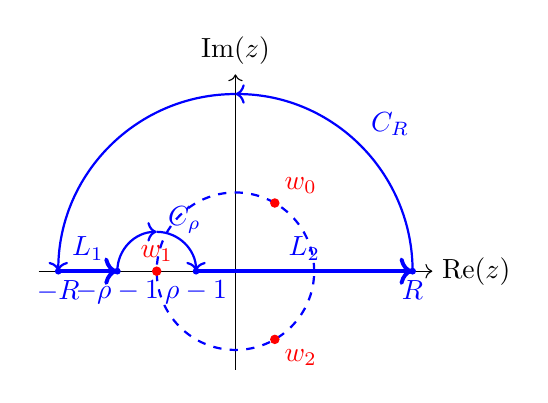
\begin{tikzpicture}[scale=1]
				% draw axes
				\draw[->] (-2.5,0) -- (2.5,0) node[right] {$\Re(z)$};
				\draw[->] (0,-1.25) -- (0,2.5) node[above] {$\Im(z)$};
				% draw unit circle
				\draw[dashed, thick, blue] (1,0) arc (0:360:1) node[] {};
				% solutions of z^3+1=0
				\filldraw[red] ({1/2},{sqrt(3)/2}) circle (1.5pt) node[anchor=south west] {$w_0$};
				\filldraw[red] (-1,0) circle (1.5pt) node[anchor=south] {$w_1$};
				\filldraw[red] ({1/2},-{sqrt(3)/2}) circle (1.5pt) node[anchor=north west] {$w_2$};
				
				% add arrow
				%\draw[->] (0,0) -- (1,1) node[midway, above left] {};
				% draw point
				\filldraw[blue] (2.25,0) circle (1pt) node[anchor=north] {$R$};
				\filldraw[blue] (-2.25,0) circle (1pt) node[anchor=north] {$-R$};
				\filldraw[blue] (-.5,0) circle (1pt) node[anchor=north] {$\rho-1$};
				\filldraw[blue] (-1.5,0) circle (1pt) node[anchor=north] {$-\rho-1$};
				
				\draw[line width=0.5mm, ->, thick, blue] (2.25,0) arc (0:90:2.25) node[midway, above right] {$C_R$};
				\draw[line width=0.5mm, ->, thick, blue] (0,2.25) arc (90:180:2.25) node[midway, left] {};
				\draw[line width=0.5mm, blue, ->] (-2.25,0) -- (-1.5,0) node[midway, above] {$L_1$};
				\draw[line width=0.5mm, blue, ->] (-.5,0) -- (2.25,0) node[midway, above] {$L_2$};
				
				\draw[line width=0.5mm, <-, thick, blue] (-.5,0) arc (0:90:.5) node[midway, above] {$C_\rho$};
				\draw[line width=0.5mm, <-, thick, blue] (-1,.5) arc (90:180:.5) node[midway, left] {};
				\end{tikzpicture}
			\end{center}
			demonstrate the following improper integral:\[
			\int_{-\infty}^{\infty}\frac{1}{x^3+1}\ dx=\frac{\pi}{\sqrt{3}}.
			\]
			\item Referring to the figure below
			\begin{center}
				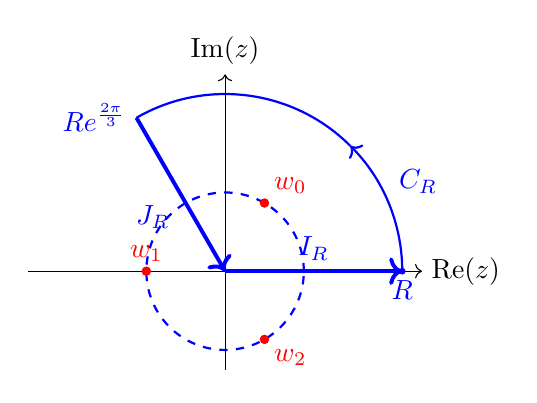
\begin{tikzpicture}[scale=1]
				% draw axes
				\draw[->] (-2.5,0) -- (2.5,0) node[right] {$\Re(z)$};
				\draw[->] (0,-1.25) -- (0,2.5) node[above] {$\Im(z)$};
				% draw unit circle
				\draw[dashed, thick, blue] (1,0) arc (0:360:1) node[] {};
				% solutions of z^3+1=0
				\filldraw[red] ({1/2},{sqrt(3)/2}) circle (1.5pt) node[anchor=south west] {$w_0$};
				\filldraw[red] (-1,0) circle (1.5pt) node[anchor=south] {$w_1$};
				\filldraw[red] ({1/2},-{sqrt(3)/2}) circle (1.5pt) node[anchor=north west] {$w_2$};
				
				% add arrow
				%\draw[->] (0,0) -- (1,1) node[midway, above left] {};
				% draw point
				\filldraw[blue] (2.25,0) circle (1pt) node[anchor=north] {$R$};
				
				\draw[line width=0.5mm, ->, thick, blue] (2.25,0) arc (0:45:2.25) node[midway, above right] {$C_R$};
				\draw[line width=0.5mm, -, thick, blue] ({2.25*sqrt(2)/2},{2.25*sqrt(2)/2}) arc (45:120:2.25) node[left] {$\displaystyle Re^{\frac{2\pi}{3}}$};
				\draw[line width=0.5mm, blue, ->] (-{2.25*1/2},{2.25*sqrt(3)/2}) -- (0,0) node[midway, below left] {$J_R$};
				\draw[line width=0.5mm, blue, ->] (0,0) -- (2.25,0) node[midway, above] {$I_R$};
				
				%\draw[line width=0.5mm, <-, thick, blue] (-.5,0) arc (0:90:.5) node[midway, above] {$C_\rho$};
				%\draw[line width=0.5mm, <-, thick, blue] (-1,.5) arc (90:180:.5) node[midway, left] {};
				\end{tikzpicture}
			\end{center}
			demonstrate the following improper integral:\[
			\int_{0}^{\infty}\frac{1}{x^3+1}\ dx=\frac{2\pi}{3\sqrt{3}}.
			\]
		\end{enumerate}\begin{proof}[\sol]
			df
		\end{proof}
		\item Demonstrate the following improper integral: \[
		\int_{-\infty}^\infty\frac{\sin x}{x^2+4x+5}\ dx=-\frac{\pi}{e}\sin 2.
		\] \begin{proof}[\sol]
			content...
		\end{proof}
		\item Demonstrate the following improper integral: \[
		\int_0^{\infty}\frac{x^2}{x^6+1}\ dx=\frac{\pi}{6}.
		\] \begin{proof}[\sol]
			content...
		\end{proof}
		\item \begin{proof}[\sol]
			content...
		\end{proof}
		\item \begin{proof}[\sol]
			content...
		\end{proof}
		\item \begin{proof}[\sol]
			content...
		\end{proof}
	\end{enumerate}
	
	\footer{Department of Information Security, Cryptography and Mathematics\\
		Collage of Science and Technology\\
		Kookmin University}
\end{document}
